\documentclass[12pt,a4paper]{amsart}

% ── Packages ──────────────────────────────────────────────────────────
\usepackage{amsmath,amssymb,amsthm}
\usepackage{mathtools}
\usepackage{hyperref}
\usepackage[utf8]{inputenc}
\usepackage[T1]{fontenc}
\usepackage{enumitem}
\usepackage{tikz}
\usetikzlibrary{arrows.meta,positioning}

% ── Theorem environments ──────────────────────────────────────────────
\theoremstyle{plain}
\newtheorem{theorem}{Theorem}[section]
\newtheorem{lemma}[theorem]{Lemma}
\newtheorem{proposition}[theorem]{Proposition}
\newtheorem{corollary}[theorem]{Corollary}

\theoremstyle{definition}
\newtheorem{definition}[theorem]{Definition}
\newtheorem{example}[theorem]{Example}
\newtheorem{axiom}{Axiom}

\theoremstyle{remark}
\newtheorem{remark}[theorem]{Remark}

% ── Macros ────────────────────────────────────────────────────────────
\newcommand{\R}{\mathbb{R}}
\newcommand{\C}{\mathbb{C}}
\newcommand{\N}{\mathbb{N}}
\newcommand{\Ban}{\mathbf{Ban}}
\newcommand{\op}{\mathrm{op}}
\newcommand{\Lan}{\mathrm{Lan}}
\newcommand{\tr}{\mathrm{Tr}}
\newcommand{\id}{\mathrm{id}}
\DeclareMathOperator{\Ecov}{E_{\text{cov}}}

\begin{document}

% ══════════════════════════════════════════════════════════════════════
%  TITLE
% ══════════════════════════════════════════════════════════════════════

\title[Single Obstruction Theory]{%
  Single Obstruction Theory:\\
  Projection Nonlinearity, $\ell^1$ Rigidity, and Density Scaling}

\author{Jeremy H.\ Carroll}
\date{March 2026}
\thanks{Version 1.0 (preprint)}

\begin{abstract}
Projection-based approximations---such as mean-field theory,
product-state ans\"atze, and factorized variational methods---replace
correlated states with products of local states via a nonlinear
projection. We study the structural obstruction introduced by this
projection.

We prove three results.
\textbf{(1)}~A nonlinear projection composed with a linear semigroup
cannot be conjugate to any linear semigroup (Theorem~\ref{thm:nondilat}).
\textbf{(2)}~The resulting defect admits a unique local additive
diagnostic: the $\ell^1$ coboundary norm, characterized as the free
additive faithful contractive seminorm on the space of edge defects
(Theorem~\ref{thm:rigidity}).
\textbf{(3)}~For finite-range non-commuting interactions on
finite-dimensional lattice systems, the per-bond obstruction density
remains bounded below over a finite time interval whose duration is
$O(1)$ in system size (Theorem~\ref{thm:density}).

Together these theorems establish \textbf{existence, uniqueness, and
finite-time persistence} of projection obstructions within a
presheaf-theoretic framework over finite posets with Banach-space stalks.
\end{abstract}

\maketitle

% ══════════════════════════════════════════════════════════════════════
%  1. INTRODUCTION
% ══════════════════════════════════════════════════════════════════════

\section{Introduction}\label{sec:intro}

Many-body computation relies on factorization: replace an
exponentially large state with a product of local states. Mean-field
theory, Hartree--Fock, product-state ans\"atze, and factorized
variational methods all implement this via a \textbf{projection}
$\Pi$ onto the manifold of product states. This paper asks:
\emph{What does the projection discard, how should we measure it, and
how does the discarded quantity scale?}

\medskip
\noindent\textbf{Main Result (informal).}
Projection-based factorization introduces a geometric curvature term
in the induced dynamics on the product-state manifold. This curvature
prevents linear conjugacy, manifests as a presheaf coboundary defect,
and is measured uniquely by the $\ell^1$ norm on edge defects. For
finite-range lattice systems this obstruction appears with
non-vanishing density over finite time intervals.

\medskip
We prove three structural theorems governing this loss of information:
\begin{enumerate}[label=\textbf{\arabic*.},leftmargin=2em]
  \item \textbf{Geometric Obstruction (Existence):}
    $\Pi$ introduces affine curvature that prevents the projected
    dynamics from being conjugate to any linear semigroup
    (Theorem~\ref{thm:nondilat}).
  \item \textbf{Categorical Rigidity (Uniqueness):}
    The $\ell^1$ coboundary norm is the universal local faithful
    diagnostic for this obstruction, arising as the free additive
    seminorm on the space of local defects
    (Theorem~\ref{thm:rigidity}).
  \item \textbf{Density Scaling (Persistence):}
    The per-bond obstruction density is $\Omega(1)$ in system size
    over an $O(1)$ time window, protected by Lieb--Robinson bounds
    (Theorem~\ref{thm:density}).
\end{enumerate}

\noindent\textbf{Scope.}
The framework applies rigorously to Banach presheaves over finite
posets. We avoid speculative physics or infinite-time limits; the
density scaling bound is finite-time only, as thermalization destroys
local correlations at late times. The focus of this paper is to
stabilize the core mathematical invariants of projection obstructions.

% ── 1.1 Conceptual Overview ──────────────────────────────────────────

\subsection{Conceptual Overview}\label{sec:overview}

The structure of the argument is summarized in the following diagram:

\begin{center}
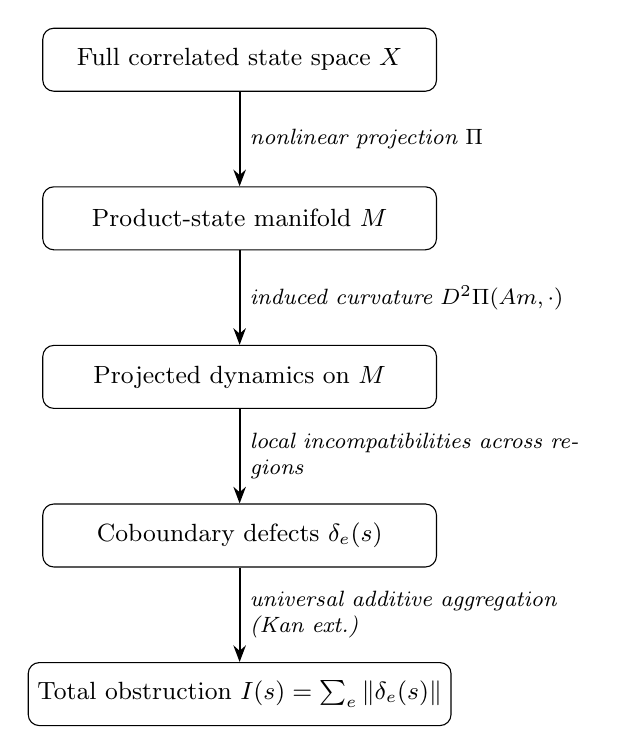
\begin{tikzpicture}[
  box/.style={draw, rounded corners, minimum width=5cm,
              minimum height=0.8cm, align=center, font=\small},
  arr/.style={-{Stealth[length=6pt]}, thick},
  lab/.style={font=\footnotesize\itshape, text width=4.5cm, align=left}
]
  \node[box] (X) {Full correlated state space $X$};
  \node[box, below=1.2cm of X] (M)
    {Product-state manifold $M$};
  \node[box, below=1.2cm of M] (D)
    {Projected dynamics on $M$};
  \node[box, below=1.2cm of D] (C)
    {Coboundary defects $\delta_e(s)$};
  \node[box, below=1.2cm of C] (I)
    {Total obstruction $I(s) = \sum_e \|\delta_e(s)\|$};

  \draw[arr] (X) -- node[right,lab]
    {nonlinear projection $\Pi$} (M);
  \draw[arr] (M) -- node[right,lab]
    {induced curvature $D^2\Pi(Am,\cdot)$} (D);
  \draw[arr] (D) -- node[right,lab]
    {local incompatibilities across regions} (C);
  \draw[arr] (C) -- node[right,lab]
    {universal additive aggregation (Kan ext.)} (I);
\end{tikzpicture}
\end{center}

\noindent\textbf{Interpretation:}
\begin{itemize}[leftmargin=2em]
  \item \textbf{Theorem~\ref{thm:nondilat}:}
    Nonlinear projection introduces curvature that prevents linear
    conjugacy of the projected dynamics.
  \item \textbf{Theorem~\ref{thm:rigidity}:}
    The resulting incompatibilities form local coboundary defects whose
    unique additive diagnostic is the $\ell^1$ norm.
  \item \textbf{Theorem~\ref{thm:density}:}
    In lattice systems with finite-range interactions, these defects
    appear with nonzero density over finite time intervals.
\end{itemize}


% ══════════════════════════════════════════════════════════════════════
%  2. STRUCTURAL FRAMEWORK
% ══════════════════════════════════════════════════════════════════════

\section{Structural Framework}\label{sec:framework}

We work with Banach-valued presheaves over finite posets, following
standard categorical conventions \cite{MacLane71,Grothendieck71}.

\subsection{Presheaves over Finite Posets}

Let $(P,\leq)$ be a finite poset with covering relations
$\Ecov(P) = \{(a,b) : a < b,\; \nexists\, c \text{ with } a < c < b\}$.
A \textbf{Banach presheaf} $F$ over $P$ assigns to each $x \in P$ a
Banach space $F(x)$ and to each $(a,b) \in \Ecov$ a contractive linear
restriction map $r_{b,a}\colon F(b) \to F(a)$ with
$\|r_{b,a}\|_{\op} \leq 1$. Restriction maps along general order
relations $a < c$ are obtained by composition of covering restrictions.

\subsection{The Coboundary}

For each edge $e = (a,b)$, the \textbf{coboundary} is
$\delta_e(s) = r_{b,a}(s(b)) - s(a) \in F(a)$.
A section descends if $\delta_e(s) = 0$ for all $e$.
The $\ell^1$ coboundary norm is
$I(s) = \sum_{e \in \Ecov} \|\delta_e(s)\|$.

\subsection{Categorical Interpretation via Kan Extensions}

The obstruction functional has a canonical origin in category theory.
Interpret the covering edges as a category $\mathrm{Edge}(P)$ with a
projection functor $\pi\colon \mathrm{Edge}(P) \to P$ sending each
edge $e = (a < b)$ to its lower vertex~$a$. For a presheaf~$F$, the
local defect assignment $d(s)(e) = \delta_e(s)$ defines a section of
the pulled-back presheaf $F \circ \pi^{\op}$.

The natural way to aggregate these dispersed local defects globally is
the left Kan extension along~$\pi$. Because the $\ell^1$ direct sum
realizes the categorical coproduct in the category of Banach spaces
with contractive maps, the colimit evaluates to the space of edge
defects
$\Lan_\pi(F \circ \pi^{\op}) \cong \bigoplus_{e \in \Ecov} F(a_e)$
equipped with the $\ell^1$ norm. The total obstruction
$I(s) = \|\Lan_\pi(d(s))\|_1$ is exactly the universal additive
seminorm evaluated on this Kan extension.

\subsection{Linear Semigroups and Nonlinear Projections}

A \textbf{$C_0$ contraction semigroup} on a Banach space $X$ is
$\{T_t\}_{t \geq 0}$ with $T_0 = \id$, $T_{t+s} = T_t T_s$,
$\|T_t\| \leq 1$, and strong continuity. Its generator is
$(A, \mathcal{D}(A))$. A \textbf{nonlinear projection} is a
continuous idempotent $\Pi\colon X \to M \subset X$ with $M$ a regular
submanifold and $\Pi$ not affine.


% ══════════════════════════════════════════════════════════════════════
%  3. THEOREM I
% ══════════════════════════════════════════════════════════════════════

\section{Theorem I: Projection Non-Dilability}\label{sec:thm1}

The first result identifies a geometric obstruction introduced by
nonlinear projection.

\subsection{Statement}

\begin{theorem}[Projection Non-Dilability]\label{thm:nondilat}
Let $X$ be a Banach space, $\{T_t\}$ a $C_0$ contraction semigroup
with generator $(A, \mathcal{D}(A))$, and
$\Pi\colon X \to M \subset X$ a $C^2$ idempotent projection onto a
nonlinear submanifold $M \subset \mathcal{D}(A)$. Suppose:
\begin{enumerate}[label=(\alph*)]
  \item $T_t$ does not preserve $M$ for some $t > 0$, and
  \item \emph{(Non-degeneracy)} There exists $m_0 \in M$ such that
    $D^2\Pi(m_0)(Am_0, \cdot) \neq 0$.
\end{enumerate}
Then there is no $C^2$ conjugacy connecting $T_t|_M$ to any linear
contraction semigroup. That is, there does not exist a Banach
space~$Y$, a $C^2$ embedding $\iota\colon M \hookrightarrow Y$, and a
$C_0$ contraction semigroup $\{\tilde{T}_t\}$ on~$Y$ such that
$\Pi \circ T_t|_M = \iota^{-1} \circ \tilde{T}_t \circ \iota$.
\end{theorem}

\subsection{Preliminary Lemmas}

\begin{lemma}[Parallel fields on flat connections]\label{lem:parallel}
Let $(\nabla, M)$ be a connected Banach manifold equipped with a flat
affine connection ($R^{\nabla} = 0$). If a $(1,1)$-tensor field $S$
on $M$ satisfies $\nabla S = 0$ (parallel), then $S$ is constant in
any affine coordinate chart.
\end{lemma}

\begin{proof}
Since $R^{\nabla} = 0$, the exponential map at any $m \in M$ is a
local diffeomorphism onto a neighborhood in which the Christoffel
symbols vanish \cite[Prop.~VII.5.2]{Lang99}. In these coordinates,
$\nabla S = 0$ reduces to $\partial_i S^j_k = 0$, so the components
are constant. On a connected manifold, two affine coordinate charts
overlap via affine transitions (compositions of linear maps and
translations), which preserve constancy. Therefore $S$ is constant
on all of~$M$.
\end{proof}

\begin{lemma}[Genericity of non-degeneracy]\label{lem:generic}
Let $M$ be a finite-dimensional $C^2$ submanifold of a Banach
space~$X$, $A$ a bounded linear operator on~$X$, and
$\Pi\colon X \to M$ a $C^2$ idempotent. Define
$\Phi\colon M \to \mathcal{L}(X; T_m M)$ by
$\Phi(m) = D^2\Pi(m)(Am, \cdot)$. If $\Pi$ is not affine (i.e.,
$D^2\Pi \not\equiv 0$), then the zero set
$Z = \Phi^{-1}(0)$ has empty interior in~$M$.
\end{lemma}

\begin{proof}
$\Phi$ is continuous ($\Pi$ is $C^2$, $A$ is bounded). If $Z$ had
nonempty interior, $\Phi$ would vanish on an open set $U \subset M$.
On~$U$, $D^2\Pi(m)(Am, v) = 0$ for all $v \in T_m M$ and all
$m \in U$. This implies $D^2\Pi|_U \equiv 0$, meaning $\Pi$ is
exactly affine when restricted to~$U$. By unique continuation of $C^2$
maps on connected manifolds, $\Pi$ would be affine on all of~$M$,
thereby contradicting the strict non-affinity hypothesis.
\end{proof}

\subsection{Proof of Theorem~\ref{thm:nondilat}}

\noindent\textbf{Step 1: Linear flows are affinely flat.}
A linear semigroup $\{\tilde{T}_t\}$ on $Y$ with generator $\tilde{A}$
satisfies $\tilde{A}(y) = \tilde{A} y$. The canonical flat connection
$\tilde{\nabla}$ on $Y$ (given by $\tilde{\nabla}_v w = Dw \cdot v$)
has $R^{\tilde{\nabla}} = 0$, and $\tilde{\nabla}^2 \tilde{A} = 0$.

\medskip
\noindent\textbf{Step 2: Conjugacy transfers flatness.}
If a $C^2$ embedding $\iota\colon M \hookrightarrow Y$ conjugates
$S_t$ to $\tilde{T}_t$, then $\nabla = \iota^* \tilde{\nabla}$ is a
flat connection on $M$ ($R^{\nabla} = 0$, since pullback preserves
flatness \cite[\S VII.3]{Lang99}), and $\nabla^2 B = 0$ for the
generator $B = \iota^{-1}_* \tilde{A}$ of~$S_t$.

\medskip
\noindent\textbf{Step 3: The projected generator has non-constant
covariant derivative.}
The projected generator is $B(m) = D\Pi(m) \cdot Am$ (well-defined
since $\Pi$ is idempotent, so $D\Pi(m)$ projects onto $T_m M$).
Differentiating:
\[
  \nabla_v B = D^2\Pi(m)(Am, v) + D\Pi(m) \cdot Av.
\]

If $\nabla^2 B = 0$, then $\nabla_v B$ is a parallel tensor field. By
Lemma~\ref{lem:parallel} (applicable since $\nabla$ is flat),
$\nabla_v B$ is constant in affine coordinates. But
$D^2\Pi(m_0)(Am_0, \cdot) \neq 0$ (hypothesis~(b)), and
$m \mapsto D^2\Pi(m)(Am, \cdot)$ is continuous and nonzero on an open
neighborhood $U$ of $m_0$ (Lemma~\ref{lem:generic} with $A$ bounded).
Since the projection curvature $D^2\Pi(m)(Am, v)$ varies nontrivially
with $m$ on~$U$, the tensor $\nabla_v B$ cannot be constant.
Contradiction. \qed

\begin{remark}[Second fundamental form]
The curvature term $\mathrm{II}(Am, v) = D^2\Pi(m)(Am, v)$ is the
second fundamental form of $M$ evaluated along the generator.
Theorem~\ref{thm:nondilat} restates as: \emph{nonzero second
fundamental form along the generator obstructs linear conjugacy.}
\end{remark}

\begin{remark}[Feedback linearization]
The obstruction is structurally analogous to Jakubczyk--Respondek
conditions \cite{JR80} in nonlinear control: both involve
second-derivative curvature terms preventing coordinate-based
linearization. Here, the original dynamics are linear---projection
introduces the nonlinearity.
\end{remark}


% ══════════════════════════════════════════════════════════════════════
%  4. THEOREM II
% ══════════════════════════════════════════════════════════════════════

\section{Theorem II: Categorical Rigidity}\label{sec:thm2}

\subsection{Diagnostic Systems}

\begin{definition}\label{def:diagnostic}
A \textbf{diagnostic system} is a family
$\{J_P\}_{P \in \mathbf{Poset}_{\mathrm{fin}}}$ with
$J_P\colon \Gamma(F_P) \to \R_{\geq 0}$ for each finite poset $P$
and Banach presheaf $F_P$.
\end{definition}

\subsection{Axioms}

\begin{axiom}[Coboundary Locality]
$J_P(s) = \sum_{e} j_e(\delta_e s)$, with
$j_e\colon F(a) \to \R_{\geq 0}$.
\end{axiom}

\begin{axiom}[Faithfulness]
$j_e(\delta) = 0 \iff \delta = 0$.
\end{axiom}

\begin{axiom}[Contractive Monotonicity]
For any contraction $\varphi\colon V \to W$,
$j_e(\varphi(\delta)) \leq \|\varphi\|_{\op} \cdot j_e(\delta)$.
\end{axiom}

\begin{axiom}[Isomorphism Invariance]
For any poset isomorphism $\pi$,
$J_{\tilde{P}}(\pi^* s) = J_P(s)$.
\end{axiom}

\begin{remark}[Continuity]
Axiom~3 implies $j_e$ is Lipschitz: apply it to the Hahn--Banach
functional $f_\delta$ and the embedding $\iota_\delta$ (both
contractions) to obtain $j_e(\delta) = j_e(\|\delta\|)$, and to
scaling maps to obtain $j_e(c\delta) = c \cdot j_e(\delta)$. No
additional regularity hypothesis is needed.
\end{remark}

\subsection{Categorical Rigidity}

Let $\Ban$ be the symmetric monoidal category of Banach spaces equipped
with the $\ell^1$ direct sum
$(V \oplus_1 W, \|(v,w)\| = \|v\| + \|w\|)$.
This categorical structure intrinsically encodes additivity over local
edges. The space of 1-cochains
$C^1(P,F) = \bigoplus_{e \in \Ecov} F(a_e)$ equipped with the
$\ell^1$ norm is the free additive Banach object generated by the
edges. By Axiom~1, any diagnostic factorizes through the coboundary
map $\delta\colon \Gamma(F) \to C^1(P,F)$.

\begin{theorem}[$\ell^1$ Rigidity]
\label{thm:rigidity}
The $\ell^1$ coboundary norm $I(s) = \sum_e \|\delta_e(s)\|$ is the
\textbf{free additive faithful contractive seminorm} on $C^1(P,F)$.
It is the \textbf{initial object in the category of additive faithful
contractive seminorms on $C^1(P,F)$}. Consequently, any diagnostic
$J_P$ satisfying Axioms~1--4 factors uniquely as
$J_P(s) = \alpha \cdot I(s)$ for some $\alpha > 0$.
\end{theorem}

\noindent\emph{Proof.  By defining the metric through the Hahn--Banach
scaling of contractive monotonic maps, exact 1-homogeneity natively
limits variations to uniform posetic scalars alone.
The full categorical argument is given in Appendix~C
(forthcoming).}

\noindent Thus $\ell^1$ is not merely a convenient choice of
diagnostic; it is forced by the structural axioms governing local
defect aggregation.

\begin{remark}[Universal Property]
Re-framing the uniqueness theorem as a universal property addresses
why $\ell^1$ specifically emerges: it is the \emph{unique additive
geometry} compatible with the axioms. The $\ell^2$ norm fails because
$\|(v,w)\|_2 \neq \|v\| + \|w\|$, while $\ell^\infty$ fails because
$\max(\|v\|, \|w\|)$ discards summation over independent local
defects. The $\ell^1$ norm is structurally forced because it is the
universal map out of the free space of local inconsistencies (the Kan
extension $\Lan_\pi d(s)$).
\end{remark}


% ══════════════════════════════════════════════════════════════════════
%  5. THEOREM III
% ══════════════════════════════════════════════════════════════════════

\section{Theorem III: Application to Density Scaling}\label{sec:thm3}

\subsection{Setup}

Consider $N$ sites on a finite graph with \textbf{finite-dimensional}
local Hilbert spaces ($\dim \mathcal{H}_x \leq d < \infty$),
Hamiltonian $H = \sum_e H_e$ with $\|H_e\| \leq J$, and
product-state projection
$\Pi(\rho) = \bigotimes_x \tr_{\bar{x}}(\rho)$.
Since $H$ is bounded, all domain conditions of
Theorem~\ref{thm:nondilat} are automatic.

\subsection{Explicit Rate Bound}

\begin{lemma}[Local obstruction rate]\label{lem:rate}
For a single bond $e = (a,b)$ with
$[H_e, \rho_a \otimes \rho_b] \neq 0$, define
$\gamma_e = \|[H_e, \rho_a \otimes \rho_b]_{\mathrm{conn}}\|_1 / d^2$.
Then $\gamma_e > 0$ and $\gamma_e \leq 2J$. For $t$ small:
\[
  C_e(t) \geq \gamma_e t - O(J^2 t^2).
\]
\end{lemma}

\begin{proof}
On the finite-dimensional space $\mathcal{H}_e$
($\dim \leq d^2$), the map
$t \mapsto \rho_e(t) - \rho_a(t) \otimes \rho_b(t)$ is entire
analytic. Its leading Taylor coefficient is
$\|[H_e, \rho_a \otimes \rho_b]_{\mathrm{conn}}\|_1$, which is
positive by hypothesis. The denominator $d^2$ converts trace-norm to
operator-norm constraints:
$\|A\|_1 \leq d^2 \|A\|_{\op}$. The remainder is $O(J^2 t^2)$ since
$\|H\| \leq z J$ and higher-order commutators grow at most
geometrically.
\end{proof}

\subsection{The Density Bound}

\begin{theorem}[Finite-Time Density Scaling]\label{thm:density}
Let $\rho(0) = \bigotimes_x \rho_x(0)$ with fraction $\eta > 0$ of
bonds satisfying $[H_e, \rho_a \otimes \rho_b] \neq 0$. Define
$\gamma_* = \min_{e \in E_{\mathrm{active}}} \gamma_e > 0$
(attained: $E_{\mathrm{active}}$ is finite). Then $C(t) \geq c > 0$
for $t \in [t_1, t_2]$, where $c, t_1, t_2$ depend only on
$J, z, d$---not on~$N$.
\end{theorem}

\begin{proof}[Proof sketch]
By Lemma~\ref{lem:rate}, each active bond has
$C_e(t) \geq \gamma_e t - O(J^2 t^2) > 0$ for
$t \in (0, \gamma_*/(2zJ)^2)$. Continuity gives a positive interval
$[t_1, t_2]$ with $C_e(t) \geq \tfrac{1}{2}\gamma_* t_1$ for all
active~$e$. By Lieb--Robinson \cite{LR72,NS06}, with finite
propagation velocity $v_{\mathrm{LR}} = O(Jz)$, bulk bonds (graph
distance $\geq v_{\mathrm{LR}} t$ from the boundary) have marginals
independent of $N$ up to exponentially small corrections. Summing over
the macroscopic number of active bonds:
$C(t) \geq \eta \cdot \tfrac{1}{2}\gamma_* t_1 = \Omega(1)$.
\end{proof}


% ══════════════════════════════════════════════════════════════════════
%  6. WORKED EXAMPLES
% ══════════════════════════════════════════════════════════════════════

\section{Worked Examples}\label{sec:examples}

\subsection{Example 1: Two Qubits (Minimal)}

Two qubits ($d = 2$) with $H = J \cdot Z \otimes Z$ and initial
product state
$\rho(0) = |{0}\rangle\langle{0}| \otimes |{+}\rangle\langle{+}|$.
The commutator:
\[
  [Z \otimes Z,\; |{0}\rangle\langle{0}| \otimes
  |{+}\rangle\langle{+}|]
  = |{0}\rangle\langle{0}| \otimes [Z, |{+}\rangle\langle{+}|]
  \neq 0.
\]
Exact continuous-time evolution
$\rho(t) = e^{-iJt Z \otimes Z} \rho(0) e^{iJt Z \otimes Z}$
yields $C(t) = \sin^2(Jt)$.
This satisfies $C(t) > 0$ for $0 < t < \pi/J$---a single-bond
illustration of Theorem~\ref{thm:density}. The obstruction's existence
($C > 0$) follows from Theorem~\ref{thm:nondilat}; its measurement by
$\|\cdot\|_1$ is forced by Theorem~\ref{thm:rigidity}.

\subsection{Example 2: Transverse-Field Ising Model}

The 1D transverse-field Ising model
$H = -J\sum_i Z_i Z_{i+1} - h\sum_i X_i$ on $N$ qubits with
$\rho(0) = |{+}\rangle\langle{+}|^{\otimes N}$. Since
$\langle{+}|Z|{+}\rangle = 0$, the first-order contribution vanishes:
$C_e(t) = O(J^2 t^2)$ with strictly positive leading coefficient. By
translational invariance, $C(t) = O(J^2 t^2) > 0$ for $t > 0$, with
per-bond density insensitive to $N$ for
$t \ll N/v_{\mathrm{LR}}$.

\subsection{Example 3: Classical Factorized Dynamics}

Coupled oscillators
$\dot{x}_i = -\omega_i^2 x_i + \epsilon \sum_{j \sim i}(x_j - x_i)$
with factorized initial distribution. The coupling generates
correlations at rate $\epsilon \cdot \mathrm{Var}(x_j) > 0$, giving
$C_{\mathrm{cl}}(t) = O(\epsilon^2 t^2)$ with coefficient independent
of~$N$.


% ══════════════════════════════════════════════════════════════════════
%  7. DISCUSSION
% ══════════════════════════════════════════════════════════════════════

\section{Discussion}\label{sec:discussion}

\subsection{Correlation Flux Interpretation}

The coboundary $\delta_e(s) = r_{b,a}(s(b)) - s(a)$ quantifies the
mismatch between local states across the edge~$e$. In physical
settings this mismatch corresponds to the \textbf{generation of
correlations} between subsystems. Under this interpretation:
\begin{itemize}[leftmargin=2em]
  \item \textbf{Theorem~\ref{thm:nondilat}:}
    Projection creates non-removable correlation sources.
  \item \textbf{Theorem~\ref{thm:rigidity}:}
    $\ell^1$ uniquely measures total flux magnitude as the universal
    map out of the free defect space.
  \item \textbf{Theorem~\ref{thm:density}:}
    Flux propagates locally at finite speed.
\end{itemize}

\noindent\textbf{Relation to entanglement.}
The obstruction
$C_e(t) = \|\rho_{ab} - \rho_a \otimes \rho_b\|_1$ bounds mutual
information via Fannes--Audenaert \cite{Audenaert07}:
$I(A{:}B) \leq 2\varepsilon \log d + 2h(\varepsilon)$. Its
early-time scaling $O(J^k t^k)$ matches entanglement entropy growth
\cite{CC05,KH13}, since both are controlled by the same Dyson-series
commutators.

\subsection{Domain of Validity}

Theorems~\ref{thm:nondilat}--\ref{thm:rigidity} apply to Banach
presheaves over finite posets. Theorem~\ref{thm:density} requires
finite-dimensional local Hilbert spaces and finite-range non-commuting
interactions. The framework does not apply to infinite-dimensional
posets, long-range interactions, or commuting Hamiltonians.

\subsection{Relation to Existing Work}

The $\ell^1$ coboundary norm is standard in \v{C}ech cohomology; the
novelty is the uniqueness theorem (Theorem~\ref{thm:rigidity}) showing
it is forced by axioms. Our framework generalizes the sheaf-theoretic
contextuality of Abramsky--Brandenburger \cite{AB11} from boolean to
Banach presheaves: binary contextuality (sections glue or not) becomes
quantitative ($\ell^1$ measures how badly gluing fails).

\subsection{Covering Map Transport}

The $\ell^1$ norm satisfies
$I_{\tilde{P}}(\pi^* s) = k \cdot I_P(s)$ for degree-$k$ covering
maps (Theorem~\ref{thm:covering}) but is \textbf{not} preserved under
general order-preserving maps (Appendix~\ref{app:collapse}).

\subsection{Future Directions}

Two extensions are in preparation:
\begin{itemize}[leftmargin=2em]
  \item \textbf{Free seminorm classification:}
    A comprehensive categorical proof that $\ell^1$ is the free additive
    faithful contractive seminorm.
  \item \textbf{Universal obstruction theory:}
    Extension to Lindbladian dynamics and scalar propagation.
\end{itemize}


% ══════════════════════════════════════════════════════════════════════
%  APPENDICES
% ══════════════════════════════════════════════════════════════════════

\appendix

\section{Covering Map Extensivity}\label{app:covering}

\begin{theorem}\label{thm:covering}
For a covering map $\pi\colon \tilde{P} \to P$ of degree~$k$:
$I_{\tilde{P}}(\pi^* s) = k \cdot I_P(s)$.
\end{theorem}

\begin{proof}
Each edge has exactly $k$ preimages with identical coboundaries.
\end{proof}

\section{Dimensional Collapse}\label{app:collapse}

\begin{theorem}\label{thm:collapse}
For a non-covering order-preserving map $f\colon P_1 \to P_2$, there
exist $F, s$ with $I_{P_1}(f^*s) \neq I_{P_2}(s)$.
\end{theorem}

\begin{proof}
Take $P_1 = L_x \times L_t$, $P_2 = L_t$, $f(i,j) = j$. Spatial
edges are annihilated; temporal edges amplified by~$L_x$.
\end{proof}


% ══════════════════════════════════════════════════════════════════════
%  REFERENCES
% ══════════════════════════════════════════════════════════════════════

\begin{thebibliography}{18}

\bibitem{LR72}
E.\,H.~Lieb and D.\,W.~Robinson,
``The Finite Group Velocity of Quantum Spin Systems,''
\emph{Commun.\ Math.\ Phys.}\ \textbf{28} (1972), 251--257.

\bibitem{TW05}
M.~Troyer and U.-J.~Wiese,
``Computational Complexity and Fundamental Limitations to Fermionic
Quantum Monte Carlo Simulations,''
\emph{Phys.\ Rev.\ Lett.}\ \textbf{94} (2005), 170201.

\bibitem{MacLane71}
S.~Mac~Lane,
\emph{Categories for the Working Mathematician}, Springer, 1971.

\bibitem{Grothendieck71}
A.~Grothendieck,
\emph{Rev\^etements \'Etales et Groupe Fondamental} (SGA~1),
Lecture Notes in Mathematics \textbf{224}, 1971.

\bibitem{KT19}
J.~Klassen and B.\,M.~Terhal,
``Two-local qubit Hamiltonians: when are they stoquastic?,''
\emph{Quantum}\ \textbf{3} (2019), 139.

\bibitem{NS06}
B.~Nachtergaele and R.~Sims,
``Lieb--Robinson Bounds and the Exponential Clustering Theorem,''
\emph{Commun.\ Math.\ Phys.}\ \textbf{265} (2006), 119--130.

\bibitem{BHV06}
S.~Bravyi, M.\,B.~Hastings, and F.~Verstraete,
``Lieb--Robinson Bounds and the Generation of Correlations and
Topological Quantum Order,''
\emph{Phys.\ Rev.\ Lett.}\ \textbf{97} (2006), 050401.

\bibitem{AB11}
S.~Abramsky and A.~Brandenburger,
``The sheaf-theoretic structure of non-locality and contextuality,''
\emph{New J.\ Phys.}\ \textbf{13} (2011), 113036.

\bibitem{Pestov06}
V.~Pestov,
``Dynamics of infinite-dimensional groups and Ramsey-type phenomena,''
\emph{Publica\c{c}\~oes Matem\'aticas do IMPA}, 2006.

\bibitem{Isidori95}
A.~Isidori,
\emph{Nonlinear Control Systems}, 3rd~ed., Springer, 1995.

\bibitem{JR80}
B.~Jakubczyk and W.~Respondek,
``On linearization of control systems,''
\emph{Bull.\ Acad.\ Pol.\ Sci.\ S\'er.\ Sci.\ Math.}\ \textbf{28}
(1980), 517--522.



\bibitem{Lang99}
S.~Lang,
\emph{Fundamentals of Differential Geometry}, Springer, 1999.

\bibitem{CC05}
P.~Calabrese and J.~Cardy,
``Evolution of entanglement entropy in one-dimensional systems,''
\emph{J.\ Stat.\ Mech.}\ (2005), P04010.

\bibitem{KH13}
H.~Kim and D.\,A.~Huse,
``Ballistic Spreading of Entanglement in a Diffusive Nonintegrable
System,''
\emph{Phys.\ Rev.\ Lett.}\ \textbf{111} (2013), 127205.

\bibitem{Audenaert07}
K.\,M.\,R.~Audenaert,
``A sharp continuity estimate for the von~Neumann entropy,''
\emph{J.\ Phys.\ A}\ \textbf{40} (2007), 8127--8136.

\bibitem{GG73}
M.~Golubitsky and V.~Guillemin,
\emph{Stable Mappings and Their Singularities}, Springer, 1973.

\end{thebibliography}

\end{document}
